% Cover letter: Business Analyst / Researcher / Operations Specialist (writing-focused AI training project), micro1
% CV: Sections/cv_business_analyst_micro1.tex -> cv_gen/2026-10-30_micro1/cv_giovanni_tauro-micro1.pdf
\documentclass[11pt,a4paper,sans]{moderncv}
% Shared preamble and header for the cover letters.
% One main file per application: cl_<company>.tex, built to
% cv_gen/coverletter_giovanni_tauro-<company>.pdf next to cv_giovanni_tauro-<company>.pdf.
% Paths (cl_gen/..., Pictures/...) are relative to the project root, as in the CV (see .latexmkrc).

\moderncvstyle{classic}
\moderncvcolor{blue}

\usepackage[scale=0.80]{geometry}
\setlength{\footskip}{136.00005pt}

\usepackage{fontawesome5}
% hyperref is loaded by moderncv itself; loading it here causes an option clash
\usepackage{xcolor}
\usepackage{graphicx}
\ifxetexorluatex
  \usepackage{fontspec}
  \usepackage{unicode-math}
  \defaultfontfeatures{Ligatures=TeX}
  \setmainfont{Latin Modern Roman}
  \setsansfont{Latin Modern Sans}
  \setmonofont{Latin Modern Mono}
  \setmathfont{Latin Modern Math}
\else
  \usepackage[T1]{fontenc}
  \usepackage{lmodern}
\fi

\usepackage[english]{babel}

% used for the PDF title and the letter closing; the visible header is \clheader below
\name{Giovanni}{Tauro}

% Header: #1 = headline under the name (same as the headline of the matching CV)
\newcommand{\clheader}[1]{%
\noindent
\begin{minipage}[c]{0.74\textwidth}
    {\Huge \textbf{Giovanni Tauro}}\\[-0.2em]
    {\small #1}\\[0.3em]

    \footnotesize
    \faMapMarker*~
    \href{https://www.google.com/maps/search/?api=1&query=Lecco+23900+Italy}
    {\color{blue}Bari-Lecco, Italy}
    \quad
    \faPhone*~
    \href{https://wa.me/393279437161}
    {\color{blue}+39 3279437161}
    \quad
    \faEnvelope~
    \href{mailto:giovanni.taurodi@gmail.com}
    {\color{blue}giovanni.taurodi@gmail.com}
    \\[-0.1em]

    \faLinkedin~
    \href{https://www.linkedin.com/in/giovanni-tauro-gt/}
    {\color{blue}LinkedIn}
    \quad
    \faGithub~
    \href{https://github.com/jotades}
    {\color{blue}GitHub}
    \quad
    \faGraduationCap~
    \href{https://scholar.google.com/citations?user=BS0aVGgAAAAJ&hl=it}
    {\color{blue}Scholar}
    \quad
    \faFilePdf~
    \href{https://www.notion.so/Giovanni-Tauro-2a7901d92f3a800b892af425c5875c6a}
    {\color{blue}Portfolio}
    \quad
    \faCubes~
    \href{https://grabcad.com/giovanni.tauro-3}
    {\color{blue}GrabCAD}

\end{minipage}
\hfill
\begin{minipage}[c]{0.18\textwidth}
    \raggedleft
    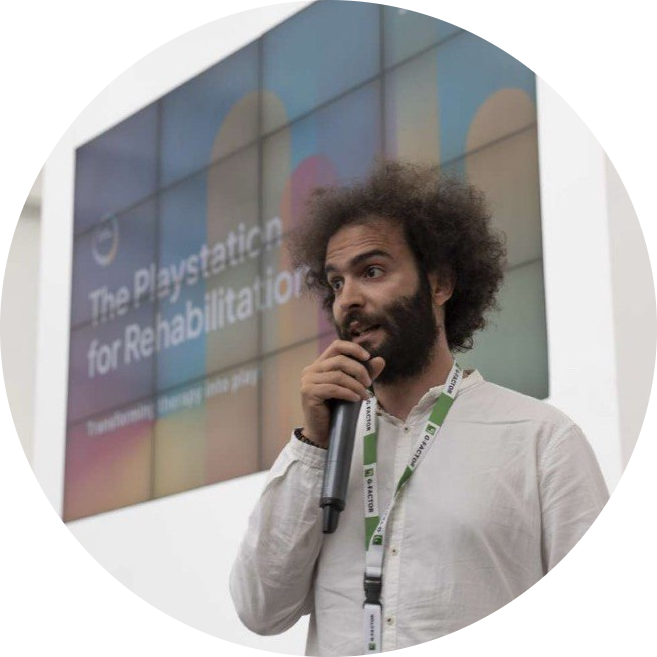
\includegraphics[width=2.8cm]{Pictures/Giovanni_pitch}
\end{minipage}
\vspace{0.1em}
}

\makeatletter
% the sender details are already in \clheader, so skip moderncv's own block
\@detailsfalse
% closing phrase, signature, name
\renewcommand*{\makeletterclosing}{%
  \@closing\\[0.6em]%
  
\includegraphics[height=1.2cm]{Pictures/sign_gt.jpg}\\[0.2em]%
  {\bfseries\@firstname~\@lastname}}
\makeatother


\begin{document}

\clheader{Business Analyst \& Researcher | Requirements, Data \& Reporting}

\recipient{micro1}{Remote}
\opening{Dear micro1 Team,}
\closing{Sincerely,}
\makelettertitle

I am applying for the Business Analyst, Researcher and Operations Specialist role on your writing-focused AI training project. I am Head of Product and co-founder of Rehabilia Technologies, and for more than five years I have worked in applied research at CNR-STIIMA, the Italian National Research Council. Most of my work ends in a written document that someone has to decide on, so judging whether an analysis or a memo really supports a decision is something I do every day.

At Rehabilia, I gather requirements through interviews with clinicians, patients and partners, map how their work is done today and turn it into specs for engineering. Our backlog is always larger than our capacity, so I weigh trade-offs with study data and user feedback, decide what enters each release and explain in writing what waits. I also run ongoing research with clinics on their needs and purchasing decisions, and I worked on our business and financial plan in the EIT Health MedTech and EIT Wildcards bootcamps.

At CNR-STIIMA, I design and run quantitative and qualitative studies: questionnaires, usability tests and interviews, with 16 blind participants for an indoor navigation system and with children with cerebral palsy, published in the \textit{Italian Journal of Pediatrics}. I analyse the data in Python and Excel and report it in papers, reports and presentations. I also designed a data tool for my research team with correction flows that keep every change traceable, a small process improvement that made our analysis easier to check.

My background is in healthcare and research rather than corporate operations, and I work with data in Python and Excel more than in SQL. The core skills are the same: asking the right questions, structuring complex information and writing clear recommendations. I use Claude and Claude Code every day and hold Anthropic's certifications for both, so I know where model output looks polished but misses the point.

I am available to work remotely on a flexible schedule, and I would welcome the chance to contribute.

\makeletterclosing

\end{document}
